\documentclass{article}

\usepackage{ctex}
\usepackage{graphicx}
\usepackage{float}
\usepackage{datetime}
\usepackage{hyperref}
\usepackage{amssymb}
\usepackage{amsthm}
\newtheorem{theorem}{Theorem}
\newtheorem{corollary}{Colollary}
\newtheorem{lemma}{Lemma}
\newtheorem{definition}{Definition}
\renewcommand\proofname{Proof}
\renewcommand\figurename{Figure}
\usepackage{listings}
\usepackage{xcolor}

\title{CS216 Assignment3 \\ {\begin{large} Applications and Variants of FFT Algorithm \end{large}}}

\author{匡亮(12111012)}

\date{April 21, 2023}

\begin{document}

\maketitle

\renewcommand\abstractname{Abstract}
\begin{abstract}

This is my report of CS216 Assignment3, including several applications of FFT:

\begin{itemize}
    \item [1.] Converting signals between time domain and frequency domain.
    \item [2.] Arbitrary-precision multiplication.
    \item [3.] More applications of FFT in sound and image processing and AI.
\end{itemize}

\end{abstract}

\newpage % contents page

\renewcommand\contentsname{Contents}
\tableofcontents

\newpage  % 1st page here

\section{Converting signals}

The core idea of this section is to look at the other viewpoint that we skipped in class.

\begin{figure}[h]  % 'h' means insert here
    \centering
    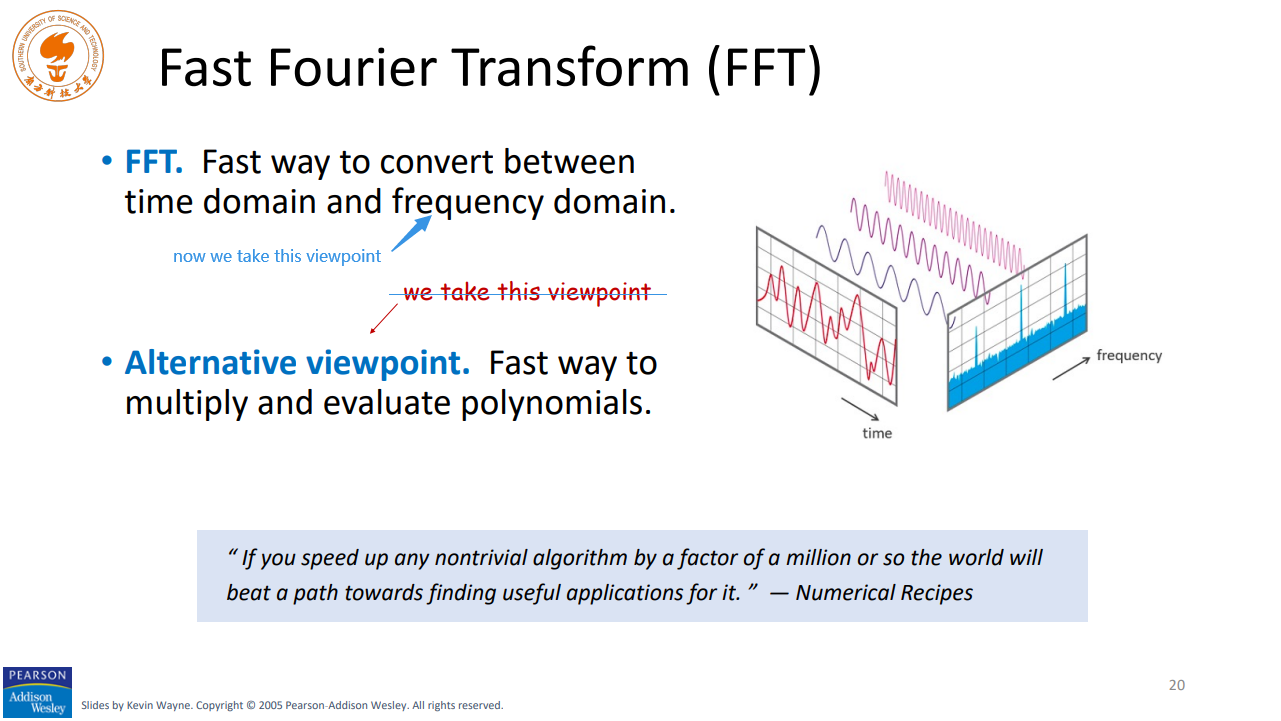
\includegraphics[height=7cm,width=11cm]{figure/1.png}
    \caption{Lecture07-dnc-multiplication-and-fft.pdf Page20}
    \label{1}
\end{figure}

A \textbf{time-domain} graph shows how a signal changes over time, whereas a \textbf{frequency-domain} graph shows how much of the signal lies within each given frequency band over a range of frequencies. A time-domain graph is often more intuitive but complex and hard to modify, so we want a quick method to change a signal between time-domain and frequency-domain.

By \textbf{fourier expansion}, we know that a period funtion $f(x)=f(x+T)$ can be expand to $f(t)=\sum_{n=-\infty}^{+\infty}c_ne^{in\omega t},c_n=\frac{1}{T}\int_{0}^{T}f(t)e^{-in\omega t}dt$. So, if our signal is the sum of some trigonometric functions with the same base frequency (i.e. their frequency are in the set $\{\omega,2\omega,3\omega,...,n\omega\}$), then, to change between time-domain and frequency-domain equals to transform between the function $f(x)$ and its corresponding sequence $c$.

Look at the two equations above, it is not hard to find that transform between $f(x)$ and sequence $c$ is DFT and IDFT, therefore we can use FFT to speed up this procedure. So far, we have a quick method to split a signal into several basic waves. In the third section we will introduce more applications of this method.

\section{Arbitrary-precision multiplication}

We have learned in the lecture that we can use FFT to convert a polynomial between its coefficient representation and point-value representation, which can speed up multiplication of two polynomials. Then if we let $x=10$ and use a polynomial to represent a large number, we can use FFT to compute the product of two large numbers. However, FFT uses floating point numbers to represent complex numbers in its calculation, which is slow, redundant and imprecise sometimes. So in this section, I will introduce a variant of FFT, called \textbf{NTT (Number-Theoretic Transform)}, which only use integer in its calcualtion.

Let's first recall why we need complex numbers in FFT. When we divide $A(x)=a_0+a_1x+a_2x^2+a_3x^3...$ into $A_{even}(x)=a_0+a_2x+...$ and $A_{odd}(x)=a_1+a_3x+...$, then calculate $A(x)$ by $A(x)=A_{even}(x^2)+xA_{odd}(x^2),A(-x)=A_{even}(x^2)-xA_{odd}(x^2)$, we want the points we chose are still pairwise negative after we squared them, which is impossible in integer domain, but possible in complex domain. However, if all coefficients in the polynomial are integers, such property is also possible in modulo domain.

By Fermat's little theorem, we konw that $a^{p-1}\equiv 1\bmod p$ when $p$ is a prime number and $0<a<p$. Similar to the FFT (where we use $\omega_n^k=e^{\frac{-2k\pi}{n}i}$), here we use $g_n^k=(G^{\frac{p-1}{n}})^k\bmod p$. To fit NTT, we have two restrictions on $p,n,G$. One is $n|(p-1)$, otherwise $\frac{p-1}{n}$ is not integer. The other is $G^i\bmod p$ shoule be pairwise different for $i\in[0,p)$, i.e. $G$ is a \textbf{primitive root} of $p$, otherwise we will have less point-values and cannot do IDFT. The prime number $p=998244353$ can perfectly fit these two restrictions in many practices, becuase it is big enough (so we will not lose any information by doing modulus), it has a primitive root $G=3$ and $p-1=2^{23}\times7\times17$, which means for $n=2^k$ where $k\le23$, $n|(p-1)$ holds, and $n=2^k$ is very convenient when doing FFT, same for NTT.

With NTT, we can do arbitrary-precision multiplication in a more elegant way, which cost less space and time, and is more precise.

\section{More applications}

\subsection{Audio editing}

If we have a song recorded in a MP3 file, which is polluted by some high frequency noise, we can use DFT to get its frequency-domain graph, eliminate the high frequency part, and use IDFT to transform it back.

\subsection{Image compression}

After applying 2-Dimension DFT on an image, for most cases, most of the values will be extremely small. Therefore, even if we only keep about top one percent of them, the 2D IDFT will give us an image very similar to the origin one. In practice, JPEG file use this method to save a lot space for image storing. If there were not FFT algorithm, this method would be unpractical because the time cost of compression and decompression would be too high.

\subsection{Computer vision}

When using CNN to reconize an image, there are plenty of convolution operation, which can be speeded up by FFT.

\section{Conclusion}

FFT is an useful and ingenious algorithm, including powerful mathematical tools and artful algorithm structure, and plays an important role in many areas of computer science. Applications of FFT is uncountable, so this report contains just the tip of the iceberg, and it worth learning for long.

\newpage

\renewcommand\refname{References}
\begin{thebibliography}{99}
    \bibitem[Reducible(2021)]{video1} The Fast Fourier Transform (FFT): Most Ingenious Algorithm Ever?

    https://www.youtube.com/watch?v=h7apO7q16V0\&t=4s

    \bibitem[Steve Brunton(2020)]{video2} The Fast Fourier Transform (FFT)

    https://www.youtube.com/watch?v=E8HeD-MUrjY\&t=2s

    \bibitem[Steve Brunton(2021)]{video3} Image Compression and the FFT

    https://www.youtube.com/watch?v=gGEBUdM0PVc
    
    \bibitem[丘比特的帽子(2022)]{video4} 硬核理解快速数论变换 Number-Theoretic Transform (NTT)

    https://www.bilibili.com/video/BV1eT411M7Fp

    \bibitem[DR CAN(2018)]{video5} 纯干货数学推导 傅里叶级数与傅里叶变换

    https://www.bilibili.com/video/BV1Et411R78v
\end{thebibliography}

\end{document}
